\documentclass{beamer}

\mode<presentation> {
	
	% The Beamer class comes with a number of default slide themes
	% which change the colors and layouts of slides. Below this is a list
	% of all the themes, uncomment each in turn to see what they look like.
	
	%\usetheme{default}
	%\usetheme{AnnArbor}
	%\usetheme{Antibes}
	%\usetheme{Bergen}
	%\usetheme{Berkeley}
	%\usetheme{Berlin}
	%%%\usetheme{Boadilla}
	%\usetheme{CambridgeUS}
	%\usetheme{Copenhagen}
	%%%\usetheme{Darmstadt}
	%%%\usetheme{Dresden}
	\usetheme{Frankfurt}
	%\usetheme{Goettingen}
	%\usetheme{Hannover}
	%\usetheme{Ilmenau}
	%\usetheme{JuanLesPins}
	%\usetheme{Luebeck}
	%\usetheme{Madrid}
	%\usetheme{Malmoe}
	%%%\usetheme{Marburg}
	%%%\usetheme{Montpellier}
	%\usetheme{PaloAlto}
	%\usetheme{Pittsburgh}
	%\usetheme{Rochester}
	%\usetheme{Singapore}
	%\usetheme{Szeged}
	%\usetheme{Warsaw}
	
	% As well as themes, the Beamer class has a number of color themes
	% for any slide theme. Uncomment each of these in turn to see how it
	% changes the colors of your current slide theme.
	
	%\usecolortheme{albatross}
	%%%\usecolortheme{beaver}
	%\usecolortheme{beetle}
	%\usecolortheme{crane}
	%\usecolortheme{dolphin}
	%\usecolortheme{dove}
	%\usecolortheme{fly}
	%\usecolortheme{lily}
	%\usecolortheme{orchid}
	%\usecolortheme{rose}
	%\usecolortheme{seagull}
	%\usecolortheme{seahorse}
	%\usecolortheme{whale}
	%\usecolortheme{wolverine}
	
	%\setbeamertemplate{footline} % To remove the footer line in all slides uncomment this line
	\setbeamertemplate{footline}[page number] % To replace the footer line in all slides with a simple slide count uncomment this line
	
	\setbeamertemplate{navigation symbols}{} % To remove the navigation symbols from the bottom of all slides uncomment this line
}


\usepackage[utf8]{inputenc}
\usepackage[ukrainian]{babel}

\usepackage{amssymb}
\usepackage{physics}


\usepackage[active]{srcltx}
\usepackage[final]{pdfpages}

\usepackage{verbatim}

\usepackage{graphicx} % Allows including images
\usepackage{booktabs} % Allows the use of \toprule, \midrule and \bottomrule in tables

\numberwithin{equation}{section}

%------------------------------------------------

 \newcommand{\tabboxl}[2]{\parbox{#1}{\vspace{0.1cm} #2 \vspace{0.1cm} }}

\newcommand{\tabboxr}[2]{\parbox{#1}{\vspace{-0.3cm}
		\begin{flushright} #2 \end{flushright} \vspace{-0.3cm} }}

\newcommand{\tabboxc}[2]{\parbox{#1}{\vspace{-0.3cm}
		\begin{center} #2 \end{center} \vspace{-0.3cm} }}

\newcommand{\liml}{\lim\limits}
\newcommand{\suml}{\sum\limits}
\newcommand{\intl}{\int\limits}

\newcommand{\inttwopi}{\intl_{0}^{2\pi}}

%----------------------------------------------------------------------------------------
%	TITLE PAGE
%----------------------------------------------------------------------------------------


\title[Short title]{Розв'язування задачі Діріхле-Неймана для рівняння Лапласа} % The short title appears at the bottom of every slide, the full title is only on the title page

\author{Бугрії Богдан, Середович Віктор} % Your name
\institute[UCLA] % Your institution as it will appear on the bottom of every slide, may be shorthand to save space
{
	Львівський національний університет імені Івана Франка \\
	Факультет прикладної математики та інформатики 
}
\date{\today} % Date, can be changed to a custom date

\begin{document}
	%------------------------------------------------
	
	\begin{frame}
		\titlepage
	\end{frame}
	
	%------------------------------------------------
	
	\begin{frame}
		\frametitle{Зміст}
		\tableofcontents
	\end{frame}

	%------------------------------------------------
	\section{Мішана задача у двозв'язній області} 
	%------------------------------------------------

	\subsection{Постановка задачі}
	
	\begin{frame}
		\frametitle{Постановка задачі}
		Нехай $D_1 \subset \mathbb{R}^2$ – обмеженна область з гладкою границею $\Gamma_1 \subset C^2$ та $D_2 \subset \mathbb{R}^2$ – обмеженна область з гладкою границею $\Gamma_2 \subset C^2$. Тоді двозв'язна область $D = D_2 \; \backslash \; \overline{D}_1$ матиме вигляд:
	
	
		\begin{figure}[h]
			\centering
			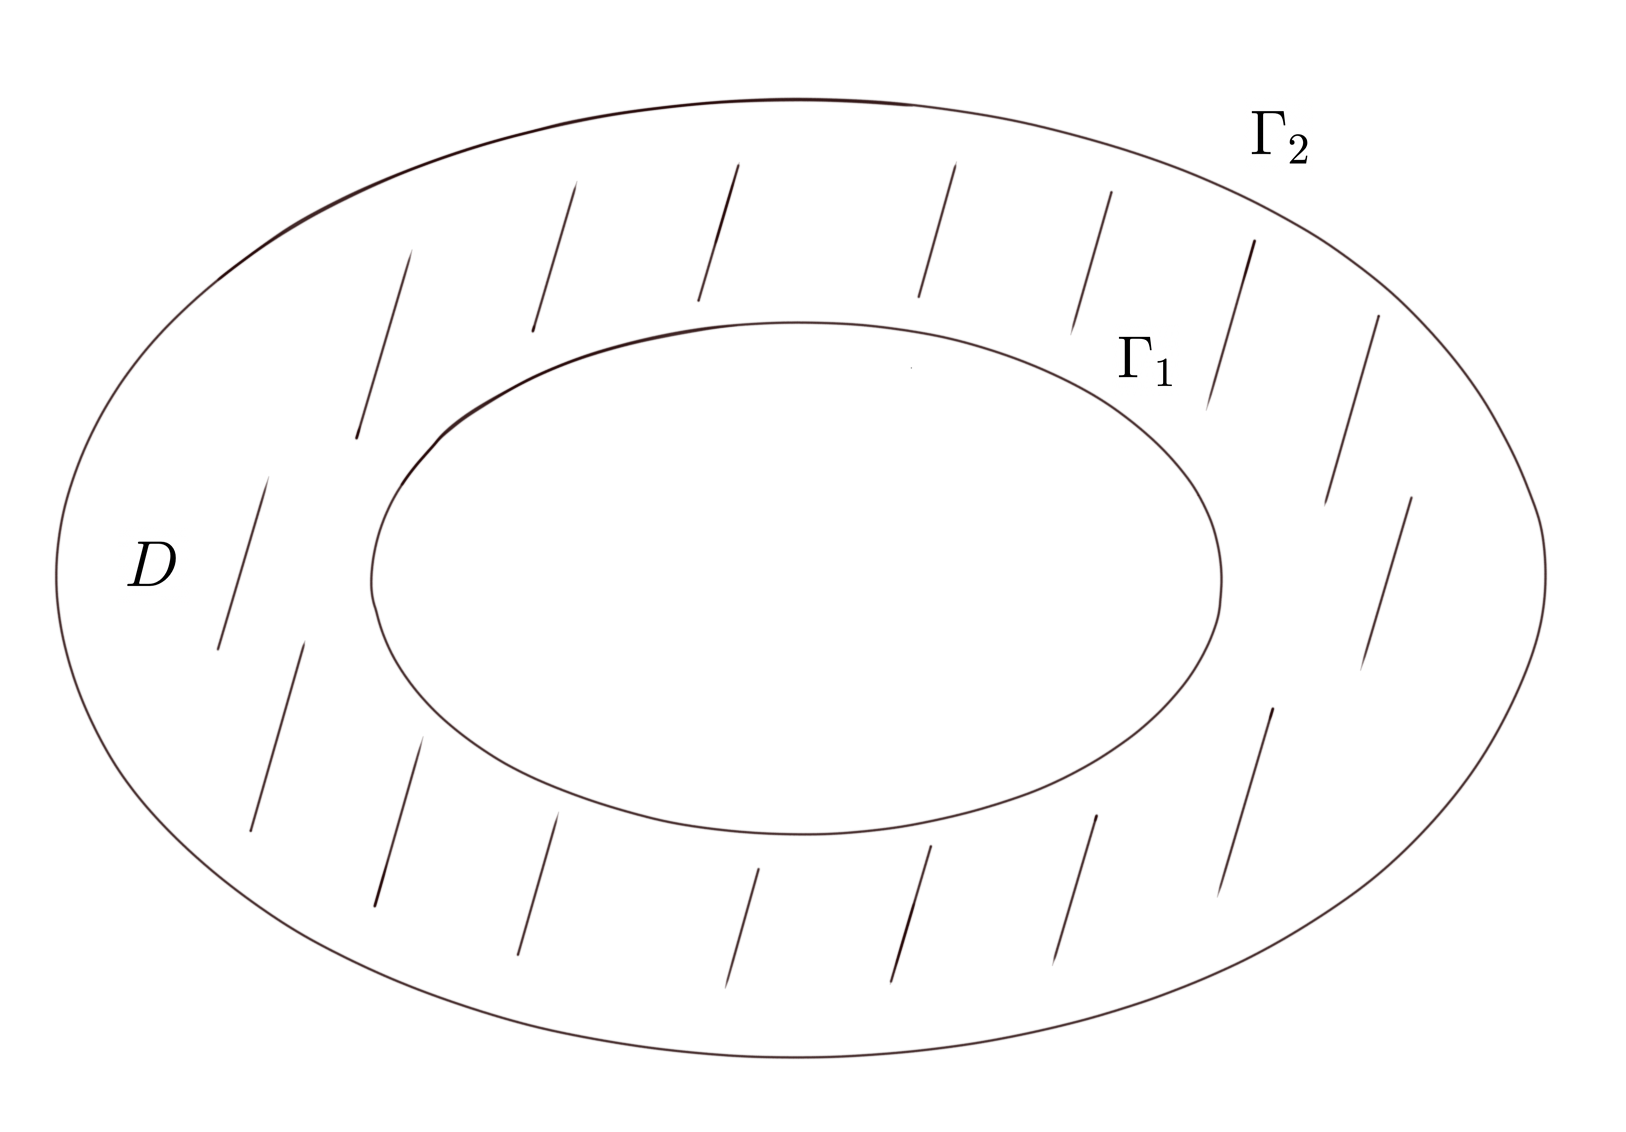
\includegraphics[width=0.6\textwidth]{resources/doubly-connected-region}
			\caption{Двоз'вязна область $D$}
			\label{fig:double-connected-region}
		\end{figure}
	\end{frame}
	
	\begin{frame}
		Задана мішана задача Діріхле-Неймана для рівняння Пуасона. Знайти таку функцію $u(x_1, x_2) \in C^{2}(D)\bigcap  C^{1}(\overline{D})$ що задовольняє рівняння (\ref{laplace-eq}) та граничні умови (\ref{dirichlet-condition}), (\ref{neumann-condition})
	
		\begin{block}{}
			
			\begin{enumerate}
				\item
				Рівняння Лапласа: 
				\begin{equation}
					\label{laplace-eq}
					\Delta{u} = 0 \quad \text{в} \quad D
				\end{equation}
				
				\item
				Граничні умови:
				\begin{equation}
					\label{dirichlet-condition}
					u = f_1 \quad \text{на} \quad \Gamma_1,
				\end{equation}
	
				\begin{equation}
					\label{neumann-condition}
					\pdv{u}{\nu} = f_2 \quad \text{на} \quad \Gamma_2,		
				\end{equation}
		
			\end{enumerate}
		\end{block}
		де $\nu = \nu(x)$ - одиничний вектор зовнішньої нормалі, (\ref{dirichlet-condition}) є умовою Діріхле, а (\ref{neumann-condition}) є умовою Неймана.

		
	\end{frame}

	%------------------------------------------------

	\subsection{Коректність}
	\begin{frame}
		\frametitle{Коректність}
	\end{frame}

	%------------------------------------------------
	\section{Зведення до системи iнтегральних рiвнянь} 	
	%------------------------------------------------

	\subsection{Подання розв'язку ІР}
	\begin{frame}
		\frametitle{Подання розв'язку ІР}
	\end{frame}

	%------------------------------------------------
	\subsection{Коректність системи ІР}
	\begin{frame}
		\frametitle{Коректність системи ІР}
	\end{frame}
	
	%------------------------------------------------
	\section{Чисельне розв'язування} 
	%------------------------------------------------
	
	\subsection{Параметризацiя та виділення особливостей} 
	
	\begin{frame}
		\frametitle{Параметризацiя та виділення особливостей}
		Припустимо, що кривi $\Gamma_{1}$ та $\Gamma_{2}$ заданi в параметричному виглядi:
		\begin{equation}
			\Gamma_{i} := \{ x_{i}(t) = (x_{i1}(t), x_{i2}(t)), \; t \in [ 0, 2\pi ] \} , \quad i = 1, 2
		\end{equation}
		\indent де $x_{i} : \mathbb{R} \rightarrow \mathbb{R}^2$, $2\pi$ періодична $\forall{t} \; \abs{x'(t)} > 0$ 
		
		Подамо систему ref в параметричному вигляді
		\begin{small}
			\begin{equation}
				\label{IE-parametrized-system}
				\left\{
				\begin{array}{l}
					\displaystyle
					\frac{1}{2\pi} \inttwopi \psi_1(\tau) K_{11}(t, \tau) d \tau
					+ \frac{1}{2\pi} \inttwopi  \psi_2(\tau) K_{12}(t, \tau) d \tau
					= g_{1}(t)
					\\ [0.3cm]
					\displaystyle
					- \frac{\psi_2(t)}{\abs{x'_{2}(t))}}
					+ \frac{1}{\pi} \inttwopi \psi_1(\tau) K_{21}(t, \tau) d \tau
					+ \frac{1}{\pi} \inttwopi  \psi_2(\tau) K_{22}(t, \tau) d \tau
					= 2g_{2}(t)
				\end{array}\right.
			\end{equation}
		
		де $\displaystyle \psi_{i}(t) = \varphi(x_{i}(t)) \cdot \abs{x'_{i}(t)}, \; g_{i} = f_{i}(x_{i}(t)), \;  i  = 1, 2; \; t \in [0, 2\pi]$ \\[0.3cm]
		
		\end{small}
	\end{frame}
	
	%------------------------------------------------
		
	\begin{frame}
		В системі (\ref{IE-parametrized-system}) ядра мають вигляд:
		$$
		\begin{array}{l}
			\displaystyle
			K_{11}(t, \tau) = \left.
			\ln{\frac{1}{\abs{x - y}}}
			\right|_{
				{\small \parbox{20mm}{$ x = x_1(t)$ \\[-4pt] $y = x_1 ({\tau})$}}
			} \quad \quad, \quad t \neq \tau
			\\ [0.8cm]
			
			\displaystyle
			K_{12}(t, \tau) = \left.
			\ln{\frac{1}{\abs{x - y}}}
			\right|_{
				{\small \parbox{20mm}{$ x = x_1(t)$ \\[-4pt] $y = x_2 ({\tau})$}}
			} \quad \quad;
			\\ [0.8cm]
			
			\displaystyle
			K_{21}(t, \tau) = \left.
			\frac{(y - x) \cdot \nu(x)}{r^2}
			\right|_{
				{\small \parbox{20mm}{$ x = x_2(t)$ \\[-4pt] $y = x_1 ({\tau})$}}
			};
			\\ [0.8cm]
			
			\displaystyle
			K_{22}(t, \tau) = \left.
			\frac{(y - x) \cdot \nu(x)}{r^2}
			\right|_{
				{\small \parbox{20mm}{$ x = x_2(t)$ \\[-4pt] $y = x_2 ({\tau})$}}
			} 
			, \quad t \neq \tau
		\end{array}
		$$		
	\end{frame}
	
	%------------------------------------------------

	\begin{frame}
		Виділяємо логарифмічну особливість для ядра $K_{11}$. За допомогою нескладних перетворень подамо його у вигляді:
		$$
		\displaystyle
		K_{11}(t, \tau) = {K_{11}}^{(1)} \ln \left(\frac{4}{e} \sin ^{2}  \frac{t-\tau}{2}\right)+{K_{11}}^{(2)}(t, \tau)
		$$
		
		$$
		\displaystyle
		{K_{11}}^{(1)}(t, \tau) =-\frac{1}{2};
		\displaystyle
		\quad \text{та} \quad
		\displaystyle
		{K_{11}}^{(2)}(t, \tau) =\frac{1}{2} \ln{\frac{\frac{4}{e} \sin ^{2} \frac{t-\tau}{2}}{\left|x_{1}(t)-x_{1}(\tau)\right|^{2}}}, \quad t \neq \tau;
		$$
		
		Для того щоб довизначити ${K_{11}}^{(2)}$, знайдему границю за правилом Лопіталя і в результаті отримаємо:
		$$
		{K_{11}}^{(2)}(t, \tau) =
		\left\{
		\begin{array}{l}
			\displaystyle
			\frac{1}{2} \ln{\frac{\frac{4}{e} \sin ^{2} \frac{t-\tau}{2}}{\left|x_{1}(t)-x_{1}(\tau)\right|^{2}}}
			,\quad t \neq \tau
			\\ [1cm]
			
			\displaystyle
			\frac{1}{2} \ln \frac{1}{e\left|x_{1}^{\prime}(t)\right|^{2}}
			,\quad  \quad  \quad  \quad   t = \tau
		\end{array}
		\right.
		$$
		
	\end{frame}

	%------------------------------------------------
	
	\begin{frame}
		Виділимо сингулярну особливість ядра $K_{22}$. Знайдемо границю при $\tau \rightarrow t$
		$$
		\lim_{\tau \rightarrow t } \pdv{\Phi(x_{2}(t), x_{2}(\tau))}{\nu(t)} =
		\frac{  x''_{2}(\tau) \cdot \nu (x_2(t)) }{ 2\abs{ x'_{2}(t)}^2 } 
		$$
		
		Отримаємо наступне параметризованне подання ядра:
		$$
		K_{22}(t, \tau) = 
		\left\{
		\begin{array}{l}
			\displaystyle
			\frac{ \left( x_{2}(\tau) - x_{2}(t) \right) \cdot \nu (x_2(t)) }{ \abs{ x_{2}(t)-x_{2}(\tau) }^2 } 
			,\quad t \neq \tau
			\\ [1cm]
			
			\displaystyle
			\frac{  x''_{2}(\tau) \cdot \nu (x_2(t)) }{ 2\abs{ x'_{2}(t)}^2 } 
			,\quad \quad  \quad  \quad  \quad  t \neq \tau
		\end{array}
		\right.
		$$
	\end{frame}

	%------------------------------------------------

	\begin{frame}
		 Подання розв'язку TODO ref в параметричному вигляді:
		$$
		u(x)=\frac{1}{2 \pi} \int_{0}^{2 \pi} \psi_{1}(\tau) K_{1}(x, \tau) d \tau+\frac{1}{2 \pi} \int_{0}^{2 \pi} \psi_{2}(\tau) K_{2}(x, \tau) d \tau, \quad x \in D
		$$
		де відповідні ядра $K_{1}$ і $K_{2}$ мають вигляд:
		$$
		K_{1}(x, \tau)=\ln \frac{1}{\left|x-x_{1}(\tau)\right|}
		\quad \text{та} \quad 
		K_{2}(x, \tau)=\ln \frac{1}{\left|x-x_{2}(\tau)\right|}
		$$
		
		
	\end{frame}

	%------------------------------------------------

	\subsection{Метод квадратур}
	\begin{frame}
			\frametitle{Метод квадратур}
	\end{frame}
		
	%------------------------------------------------
	
	\subsection{Похибка}	
	\begin{frame}
		\frametitle{Похибка}
	\end{frame}
	
	%------------------------------------------------

	\section{Чисельні експеременти} 

	\begin{frame}
		\frametitle{Чисельні експеременти}
	\end{frame}
	
	%------------------------------------------------
	
\section*{Література}
\begin{frame}
	\thispagestyle{empty}
	\frametitle{Література}
	\begin{thebibliography}{99}
		\bibliographystyle{plain}

		\bibitem{l1}{\it Kress R.}
		Linear Integral Equations, 2nd. ed. / R. Kress. -- 
		New-York: Springer-Verlag, 1989. -- 367 с.

		\bibitem{l2}{\it Абрамовиц М.}
		Справочник по специальным функциям / М. Абрамовиц, И. Стиган. 
		-- М.: Наука, 1979. -- 832 с.
		
		\bibitem{l2}{\it Chapko R., Johansson B.T. }
		An alternating boundary integral based method for inverse potential flow around immersed bodies, No. 1, 2009
		
	\end{thebibliography}
\end{frame}

	
	%------------------------------------------------	
	
	\begin{frame}

		\frametitle{Table}
		\begin{table}
			\begin{tabular}{l l l}
				\toprule
				\textbf{Treatments} & \textbf{Response 1} & \textbf{Response 2}\\
				\midrule
				Treatment 1 & 0.0003262 & 0.562 \\
				Treatment 2 & 0.0015681 & 0.910 \\
				Treatment 3 & 0.0009271 & 0.296 \\
				\bottomrule
			\end{tabular}
			\caption{Table caption}
		\end{table}
	\end{frame}
	
	%----------------------------------------------------------------------------------------
	
\end{document} 